% This is samplepaper.tex, a sample chapter demonstrating the
% LLNCS macro package for Springer Computer Science proceedings;
% Version 2.20 of 2017/10/04
%
\documentclass[runningheads]{llncs}
%
\usepackage{cite}
\usepackage{amsmath,amssymb,amsfonts}
\usepackage{graphicx}
\usepackage{textcomp}
\usepackage{xcolor}
\usepackage{subfigure}
\usepackage{algpseudocode}
\makeatletter
\renewcommand{\ALG@beginalgorithmic}{\small}
\makeatother
\usepackage{algorithm}
\usepackage{multirow}
\usepackage{longtable}
\usepackage{booktabs, colortbl, tabularx}
\usepackage{flushend}
\usepackage{todonotes}
% Used for displaying a sample figure. If possible, figure files should
% be included in EPS format.
%
% If you use the hyperref package, please uncomment the following line
% to display URLs in blue roman font according to Springer's eBook style:
% \renewcommand\UrlFont{\color{blue}\rmfamily}

\begin{document}
%
\title{StocNoC:Accelerating Stochastic Models through Reconfigurable Network on Chip Architectures}
%
%\titlerunning{Abbreviated paper title}
% If the paper title is too long for the running head, you can set
% an abbreviated paper title here
%
\author{Arshyn Zhanbolatov \and
Kizheppatt Vipin\orcidID{0000-0002-1013-7727} \and
Aresh Dadlani\orcidID{0000-0001-6841-9682} \and
Dmitriy Fedorov}
%
\authorrunning{A. Zhanbolatov et al.}
% First names are abbreviated in the running head.
% If there are more than two authors, 'et al.' is used.
%
\institute{Department of Electrical and Computer Engineering, Nazarbayev University, Nur-Sultan, Kazakhstan 010000\\
\email{arshyn.zhanbolatov@nu.edu.kz}}
%
\maketitle              % typeset the header of the contribution
%
\begin{abstract}
%\fontdimen2\font=0.54ex
Spreading dynamics of many real-world processes lean heavily on the topological characteristics of the underlying contact network. 
With the rapid temporal and spatial evolution of complex inter-connected networks, microscopic modeling and stochastic simulation of individual-based interactions have become challenging in both, time and state space. 
Driven by the surge to reduce the time complexity associated with system behavior analysis over different network structures, we propose a network-on-chip (NoC) based FPGA solution called StocNoC.
The proof of concept is supported by the design, implementation and evaluation of the classical heterogeneous susceptible-infected-susceptible (SIS) epidemic model on a scalable NoC.
The steady-state results from the proposed implementation for the fractions of susceptible and infected nodes are shown to be comparable to those acquired from software simulations, but in a significantly shorter time period. 
Analogous to network information diffusion, implementation of the SIS model and its variants will be beneficial to foresee possible epidemic outbreaks earlier in time and expedite control decisions.
\end{abstract}
\section{Introduction}
\label{sec:intro}

Epidemic modeling is an effective mathematical tool widely adopted in many domains to quantify the spreading dynamics of processes intertwined with large-scale networks~\cite{Vynnycky2010}. It serves as a viable framework for analyzing information diffusion in social networks~\cite{Dadlani2017}, cascading failure in power grids~\cite{Korkali2017}, secure routing in communication networks~\cite{Cheng2017}, and digital virus spreading in wireless mobile networks~\cite{Yang2018}. Dynamical models at the network scale can be broadly classified into two types: \emph{deterministic} and \emph{stochastic}. In deterministic models, the network is divided into smaller groups, each representing a specific stage of the epidemic. Such models, often formulated as differential equations (in continuous time) or difference equations (in discrete time), abstract what happens on the average at the network level. In contrast, a stochastic model is formulated as a stochastic process which in turn, is a set of random variables, $X(t;\varpi) \!\equiv \! X(t)$, defined as $\{X(t;\varpi)| t \!\in T~\textrm{and}~\varpi \!\in \!\Omega\}$ where $T$ and $\Omega$ represent time and a sample space, respectively. The solution of a stochastic model is a probability distribution for each of the random variables. Such models allow follow-up of each node in the network randomly~\cite{Brauer2001,Britton2010}.

Evolution of natural and man-made networks in both scale and complexity has triggered interdisciplinary research on characterizing the dynamics of stochastic processes spreading over them. 
Similar to the spreading of pathogens in biological systems, the virulence of spreading processes depends not only on the infection rate of each node, but also on the connectivity of the underlying network structure~\cite{Mieghem2014}. Increase in computational power over recent years has revealed the existence of heterogeneous and multi-faceted relations in the description of various diffusion processes~\cite{Newman2018}. %Limited mainly by memory space, the integration of such complex features in understanding the course of epidemic outbreaks using sophisticated simulation tools becomes time demanding as the network grows in size. 
The time taken to project the spreading pattern is important in devising effective countermeasures to prevent any potential outbreaks.
\begin{figure}[t!]
    \begin{center}
    \includegraphics[width=0.8\columnwidth]{Figures/SIS.pdf}
    \caption{Schematic of the SIS model where $A_i$ denotes the direct neighbors of node $i$ in the network adjacency matrix $A$.} 
    \label{figure:sis}
    \end{center}
    \vspace{-5mm}
\end{figure}

We propose a network-on-chip (NoC) model supported on a reconfigurable platform called StocNoC to accelerate the epidemic projection of the spreading model. Due to its inherent parallelism, hardware implementation may significantly outperform pure software implementation especially due to the concurrent friendly nature of the model. The model is easily scalable to support larger network sizes, only limited by the resource availability of the target FPGA devices. Recent introduction of FPGA-accelerators in the cloud environment is especially encouraging in this regard, where users can choose the target device and scale it based on their computing requirements~\cite{Parimal2018}. Since the cloud-model charges users based on the target platform type and their running time, accelerated computation can significantly reduce the cost of computation. With minor modifications, the proposed platform can be used for hardware acceleration of other epidemic spreading models as well as spreading dynamics in contact networks in general.

The remainder of this paper is organized as follows. Section~\ref{sec:related} discusses the background of epidemic models and related works. Section~\ref{sec:architecture} presents the detailed architecture of the proposed hardware platform. Section~\ref{sec:results} discusses the hardware implementation results and the comparison with corresponding software implementation and Section~\ref{sec:conclusion} finally concludes the paper and gives future research directions.

\section{Background and Related Works}
\label{sec:related}
Epidemic models are used to predict the progression of infectious diseases in a given population and the likely outcome of an epidemic. 
%The existing spectrum ranges from coarse population-based models to detailed agent-based models. 
The classical susceptible-infected-susceptible (SIS) model depicted in \figurename{~\ref{figure:sis}} serves as the basis for many extended models, wherein $S_i(t)$ and $I_i(t)$ denote the probability of node $i$ being in the susceptible ($S$) or the infected ($I$) state, respectively, in a network of size $N$ \cite{Vynnycky2010}. Nodes that recover from the infection immediately transition to being susceptible again. The discrete-time node-level SIS epidemic model has the following form:
\begin{align}
	S_i(t) = \beta S_i(t-1) \sum_{j=1}^N a_{i,j} p_j(t) - \gamma p_i(t),
\end{align} 
satisfying the condition $S_i(t) + I_i(t) = 1$ for all $t$ values. Here, $\beta$ denotes the rate at which node $i$ gets infected, $\gamma$ is the recovery rate, $p_i$ is the probability of $i$ being infected at time $t$, and $a_{ij}$ is any element in the adjacency matrix $A$ corresponding to the network defined as:
\begin{align}
    A =\! \{a_{ij}\} \!=\! 
\begin{cases}
    1,   & \text{if } \text{nodes \emph{i} and \emph{j} are connected neighbors}\\
    0,   & \text{otherwise}.
\end{cases}
\end{align}

Advancements in network science led to the revival of several unique recurring patterns inherent in networks which essentially drive the spreading pattern of processes. The Erd\"{o}s-R\'{e}nyi (ER) model was the first to be used for generating typical random networks \cite{Erdos60onthe}. 
%Although having limited realistic applications, the model serves as a benchmark for many studies due to its interesting characteristics. 
An ER network of $N$ nodes, wherein a link is included independent of other links with probability $p$, has a mean link count of $\binom{N}{2} p$, mean degree of $(N-1)p$, and binomial degree distribution. Such networks manifest low degree heterogeneity (most nodes have the same degree), low clustering coefficient (probability that two neighbors of a node are also neighbors), and short average path length.
While ER networks are highly robust against deliberate attacks, they lack the large degree of transitivity witnessed in reality. To overcome this shortcoming, the Watts-Strogatz (WS) model was proposed to generate random graphs with small-world properties by rewiring the links of a lattice with some given probability \cite{barabasi2016network}.
This model is built on the interpolation between a standard ER random graph and a network with maximal clustering.
The Barab\'{a}si-Albert (BA) model was then developed to generate random scale-free networks with high degree heterogeneity. Based on the concept of preferential attachment or ``the rich gets richer'', the network initially begins with at least two nodes where a newly added node is most likely to connect to nodes with higher degrees. This results in the formation of a few highly-connected nodes in the network. The resulting network degree distribution has no characteristic scale as they have power law tail. Unlike ER networks that exhibit an average distance of $\log(n)$, scale-free BA networks are ultra small-world networks with a sub-logarithmic small diameter proportional to $\log(\log(n))$ and thus, are particularly robust against random node failures.

\begin{figure}[!t]
    \begin{center}
    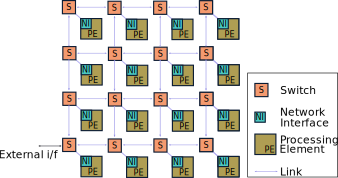
\includegraphics[width=0.6\columnwidth]{Figures/noc.pdf}
    \caption{Proposed NoC-based platform with mesh topology showing switch interconnections and network interfaces.} 
    \label{figure:noc}
    \end{center}
    \vspace{-8mm}
\end{figure}


Except for a few, most of the existing simulation tools support deterministic modeling of simplified processes. EpiModel \cite{Jenness2018} is an R package to analyze stochastic individual and network-level epidemic models. A stochastic simulator for generalized epidemic modeling known as GEMFsim \cite{SAHNEH201736} has been reported and made available in MATLAB, R, Python, and C programming platforms. These simulators however, demand longer running time as the scale and complexity of the network increases.
%\todo[inline]{If possible please shorten the description of different network models and fit into a single para. Rather explain why these different models are significant in modeling. Also a few lines on the traditional approach of modeling, like they are modeled using modeling software such as Matlab and Simulink. This might give a motivation to apply hardware acceleration.}

In this work, we propose to emulate the SIS process on an NoC platform.
NoC is an interconnect approach that helps different subsystems in a system to communicate with each other in a scalable manner~\cite{Dally2003}.
In this approach, each processing element (PE) is connected to a switch and multiple switches are interconnected to form a network.
They follow packet switched communication paradigm which makes them highly scalable.  
In the past, NoCs have been successfully used in many applications including image and signal processing~\cite{Joshi2007}, neural networks~\cite{Furber2013}, multi-processor systems~\cite{Bertozzi2005}, and virtual machines~\cite{Mathias2006}.
To the best of our knowledge, this is the first application of NoCs for accelerating stochastic models.

Due to the inherent similarity in architecture, NoCs appear to be ideal candidates for mapping different network models encountered in spreading models.
In the past, FPGAs in general and NoCs in particular have not been explored for modeling stochastic network models.
The overall aim of this work is to introduce the FPGA community the possible application of FPGA-based NoCs in accelerating dynamics of spreading models. It is not limited to epidemics but to other spreading networks including social media. 
%The current design is available as open source to attract more researchers in this direction. 

\begin{figure}[t!]
    \begin{center}
    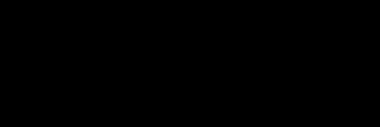
\includegraphics[width=0.75\columnwidth]{Figures/packet_format.pdf}
    \caption{Different packet formats to support network configuration and data communication.} 
    \label{figure:pktformat}
    \end{center}
    \vspace{-8mm}
\end{figure}
\section{Architecture}
\label{sec:architecture}
StocNoC follows mesh topology with each processing element (PE) along with its network interface (NI) representing a \emph{node} in the contact network.
Nodes are interconnected with the help of switches and bi-directional physical links as shown in~Fig.~\ref{figure:noc}.
The NoC configuration and inter-node communication are supported via packet switching.
The bottom left switch acts as the communication interface with external world, through which configuration packets are sent as well as the network status is monitored.
An external host such as a server computer configures the NoC for the target network and monitors the network status as time progresses. 
By analyzing the packets received from the network, the host can determine the specific nodes that are infected, nodes that have recovered, and the overall spreading pattern of the process.



\subsection{Packet Formats}
StocNoC manages configuration as well as inter-node communication using the different packet formats shown in Fig.~\ref{figure:pktformat}.
It supports unicast, multicast and broadcast packet transmissions based on the packet~\emph{type}. 
Unicast packets are used for node configuration~(at zero epoch or at $t = 0$) by an external host. 
The target node address (X and Y coordinates of the node) is stored in the \emph{destination address} field and the configuration data are carried in the \emph{input number (in)} and \emph{initial status (is)} fields. 
The \emph{input number} configures the number of neighbors (number of nodes connected to this node based on the adjacency matrix) and the \emph{initial status} configures whether the node is infected or susceptible at zero epoch.

Multicast packets are used for inter-node communication, where each node updates all its neighbors with its status after each epoch (each discrete time in simulation).
Rather than sending the same packet to each of its neighbors, each node injects a single packet to the NoC and the unique router design duplicates the packets close to the target nodes.
This considerably reduces the network routing congestion and improves the overall latency.
The packet carries the address of the injecting node in the \emph{source address} field and the status (infected/susceptible) in the \emph{status (s)} field.
Due to the packet switched nature of the NoC, it is possible that packets are delivered out-of-order to the destination nodes.
To manage this, each multicast packet carries a \emph{sequence number (sn)} field, which specifies the discrete simulation time.
Every packet in the network originating at the same discrete simulation time will have the same sequence number.

Since all nodes in the network share the same infection~($\beta$) and recovery rates~($\gamma$), this information is broadcasted across the network at the beginning of the simulation. 
Again, the router design and the routing algorithm enables injecting a single packet from the external host and the packet being replicated and delivered to each node.
The \emph{rate segment} of the packet initializes a portion of the pseudo random binary sequence (PRBS) generator used in the network interface discussed in Section~\ref{sec:ni}.
Since the current implementation uses a 100-bit long PRBS and the rate segment is only 10-bits wide, 10 configuration packets are required to initialize them. 
NoC configuration packets are special broadcast packets that configure the routing tables~(RTs) inside the switches. 
Each packet configures a portion of an RT and multiple packets are required to configure the entire network.
\begin{figure}[t!]
	\begin{center}
    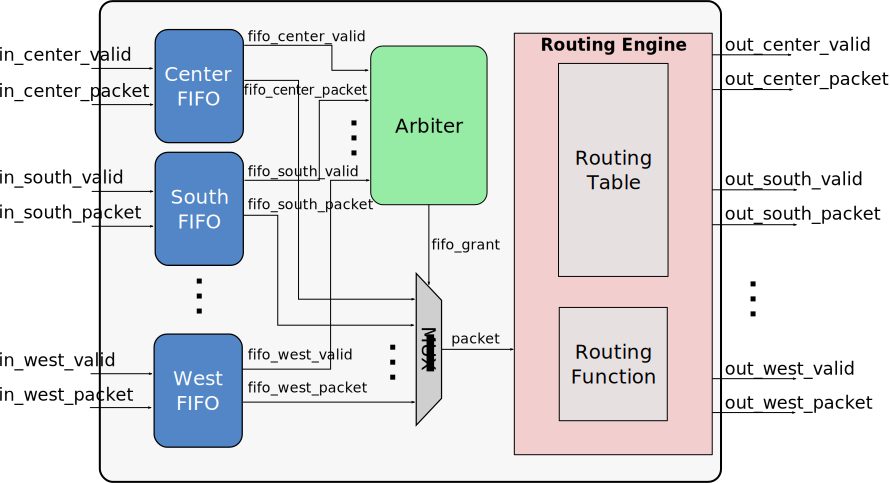
\includegraphics[width=0.8\columnwidth]{Figures/ROUTER.pdf}
    \caption{The NoC switch architecture with store-and-forward functionality and support for unicast and multicast routing.} 
    \label{figure:router}
    \end{center}
    \vspace{-5mm}
\end{figure}

\subsection{Switch}
The overall architecture of the StocNoC switch is depicted in Fig.~\ref{figure:router}.
The switch follows store and forward architecture with each interface (from 4 neighboring switches and the node) connected to an input FIFO.
Every switch interface follows AXI4-Stream protocol~\cite{xilinxaxi}.
To limit resource utilization, output FIFOs are omitted in the design.
An arbiter chooses one of the input FIFOs for packet transmission based on their requests following a round-robin scheme.
This avoids resource starvation and minimizes packet queueing delays. 
The \emph{fifo\_grant} signal from the arbiter drives the output of a multiplexer which selects the appropriate FIFO output for packet transmission. 

The selected packet is forwarded to the routing engine~(RE).
The RE logic first checks for the packet type.
Unicast packet~(PE configuration packets) routing is managed by a routing function (RF) and multicast packet~(PE status packets) routing is managed by a routing table~(RT).
The RF logic implements the traditional dimension-ordered XY routing by comparing the destination address embedded in the packet with the switch's address~\cite{Chawade2012}.

Multicast routing scheme is deployed for status packets to reduce the network congestion and latency.
This method also frees nodes from storing the RTs thus, making their design relatively simple.
A node sending its status puts only its source address into the packet and injects to the corresponding switch, unaware of the packet's ultimate targets.
Each entry in the RT used for multicast routing is 5 bits wide and the RT depth is same as the overall network size~(number of nodes in the network).

The source address embedded in the multicast packets serves as the RT entry number.
Each bit in a table entry determines the directions in which a packet originating from the corresponding address will be forwarded.
The broadcast could be to one or more of the neighboring switches as well as the to the node interfaced with the switch.
By appropriately configuring the RTs, packets from any node can be broadcasted to any given subset of nodes within the network. 
The routing path taken by each packet is similar to \emph{tree routing}, where the root of a tree is the source node and the destination nodes are located at the tree branches and leaves. 
If the destination nodes are located along the tree branches, intermediate switches perform forward-and-absorb operation. 
Traditional tree routing suffers from the possibility of deadlocks~\cite{Samman2010} in the intermediate nodes, but combining it with XY routing circumvents this possibility. 

\begin{figure}[t!]
    \begin{center}
    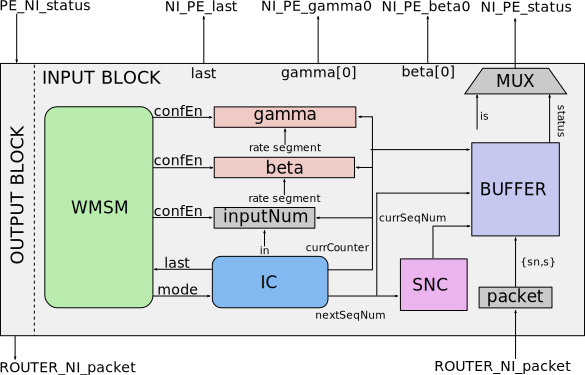
\includegraphics[width=0.8\columnwidth]{Figures/NI.pdf}
    \caption{Network Interface Architecture.} 
    \label{figure:ni}
    \vspace{-5mm}
    \end{center}
\end{figure}

The content of each RT is determined offline by an application based on the network adjacency matrix. 
For a network with \emph{NETWORK\_SIZE} nodes, aspect ratios \emph{X} and \emph{Y}, and adjacency matrix \emph{adjacencyMatrix[NETWORK\_SIZE]$\\*$[NETWORK\_SIZE]}, each table entry \emph{i} corresponding to each switch \emph{j} is generated based on Algorithm~\ref{algo}. 
The entire RT is injected to the network through the bottom-left switch as NoC configuration broadcast packets.
This approach is taken to keep packets sizes small, as packets do not carry information regarding router and RT address. 
From the received broadcast packets, each switch selects only the portions corresponding to its RT and transmits the entire table to the neighboring switch to its right.
Switches along the first column of the NoC transmits these packets to the neighboring switches in the north direction as well.
The switch's knowledge about its own address and an internal packet counter enables this configuration strategy.
Each packet carries only a fraction of the table (10-bits or 2 entries) and may require thousands of packets for complete configuration.
\begin{algorithm}[!t]
	\caption{Routing Table Generation}
	\begin{algorithmic}[1]
		\State Clear all RT entries.
		\For{j =0; j$\textless$NETWORK\_SIZE; j=j+1}
     		\For{i =0; i$\textless$NETWORK\_SIZE; i=i+1}
         		\If{adjacencyMatrix[j][i]==1}
             		\State inAddr=i;
             		\State outAddr=j;
             		\State RT[i][j][CENTER] = 1;
            		\If{outAddr [X]$\textgreater$ inAddr [X]}
                		\For{x=outAddr[X]; x$\textgreater$inAddr[X];x=x-1}
                    		\State RT[outAddr[Y]$\times$XSIZE+x][j][WEST]=1
                		\EndFor
             		\Else
                		\For{x=outAddr[X];x$\textless$inAddr[X];x=x+1}
                    		\State RT[outAddr[Y]$\times$XSIZE+x][j][EAST]=1
                		\EndFor
            		\EndIf
             		\If{outAddr[Y]$\textgreater$inAddr[Y]}
                		\For{y=outAddr[Y];y$\textgreater$inAddr[Y];y=y-1}
                   			\State RT[y$\times$XSIZE+inAddr[X]][j][SOUTH]=1
                		\EndFor
             		\Else
             			\For{y=outAddr[Y];y$\textless$inAddr[Y];y=y+1}
                    		\State RT[y$\times$XSIZE+inAddr[X]][j][NORTH]=1
                		\EndFor
             		\EndIf
         		\EndIf
     		\EndFor
 		\EndFor
\end{algorithmic}
\label{algo}
\end{algorithm}
\setlength{\textfloatsep}{15pt}

\subsection{Network Interface (NI)}
\label{sec:ni}

The NI module manages the communication between a switch and the corresponding PE. Moreover, it also implements the logic to control the state of the node after each discrete simulation time.
Its detailed architecture is depicted in Fig.~\ref{figure:ni}.
The \emph{working mode state machine} (WMSM) manages the operating mode of a node, which may be either in \emph{configuration state} or in \emph{running state}.
When the network is in the configuration state, WMSM routes the configuration packets received from the switch interface to appropriate destination registers.
The contents of the unicast packet specifying the number of neighbors of the node is stored in the \emph{inputNum} register.

The discrete time probabilities required to decide the state of a node (whether infected or susceptible) are implemented by the \emph{gamma} and \emph{beta} PRBS generators.
Both are linear feedback shift registers (LFSRs) composed of $100$ flip-flops with the last stage feeding back to the first stage.
In order to implement a specific rate (infection or recovery), the corresponding probability is multiplied by $100$ and the LFSR is initialized with a random binary pattern with number of ones equal to the result of multiplication. 
For example, to achieve a $\beta$ value of $0.3$, the $100$ flip-flops in the \emph{beta} LFSR are initialized with a random binary pattern with $30$ ones and $70$ zeros.
The initialization values for the two PRBS generators are received as broadcast packets from the external host.
Since the size of PRBS generators is much larger than the packet size, multiple configuration packets are required to initialize them.
The \emph{Input Counter (IC)} logic specifies the index number of the PRBS generators to which the incoming configuration packet values are written.
%The WMSM routes the initialization data to the appropriate PRBS based on the status signals from IC.


After initialization, the LSFRs freely run and the least significant bit (LSB) is used for achieving the required rate.
Due to the initialization pattern, the probability of the LSB becoming one will be same as the required rate.
This is similar to finding a number between $0$ and $1$ from a uniform distribution and checking whether its value is less than the required rate.
This software approach is emulated in hardware through the said mechanism.
The initialization patterns are generated offline through a software application and broadcasted to the nodes through multiple packets as discussed before.
Although same initialization packets are broadcasted to all the nodes, due to the inherent latency in packet switching, each LFSR will have a different initialization pattern at epoch zero but representing the same rate.

Once the WMSM receives the unicast packet carrying the initial node status, it is transferred to the PE and is switched to \emph{running state}. 
When a PE receives its initial status, it is immediately broadcasted to its neighbors.
Thus,some PEs may possibly receive packets from its neighbors before the end of the configuration. 
Moreover, due to path length differences and different congestion levels along different paths, out-of-order packets may arrive even at running state which may result in a node receiving a status from one of its neighbors for the next discrete time before receiving all status for the current time. 


\begin{figure}[t!]
    \begin{center}
    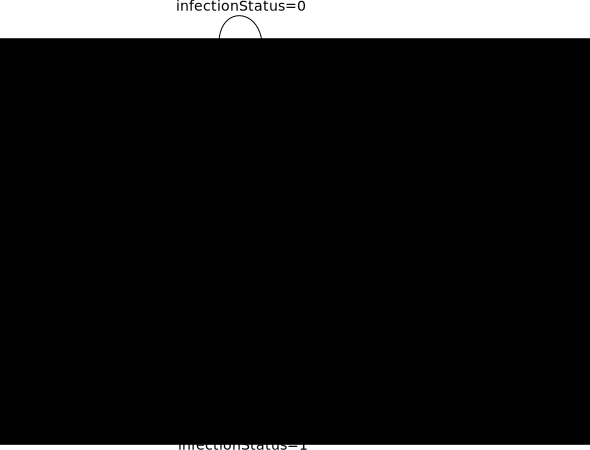
\includegraphics[width=0.7\columnwidth]{Figures/ISSM.pdf}
    \caption{SIS State machine} 
    \label{figure:fsm}
    \end{center}
    \vspace{-5mm}
\end{figure}

To overcome the out-of-order status delivery, PEs embed a sequence number into the status packets.
The sequence number indirectly represents the current discrete time.
When status packets are received, they are initially stored in a buffer with logical partition for each sequence number.
Each partition can store NETWORK\_SIZE number of status and each entry is just one $1$ bit wide (to represent infected or susceptible).  
Each partition maintains its own counter which counts the number of status that have already arrived and to which entry the next status will be updated. 
In running mode, the status are extracted from a partition specified by the \emph{sequence number checker} (SNC) one at a time and transferred to the PE.
The status are sent to the PE only after receiving the status from all its neighbors, whose number is specified in the \emph{inputNum} register during configuration.
Once all status are sent, the SNC is incremented to select the next partition.
Since each PE generates a status packet only after receiving the status from all its neighbors, it could be proven that two sequence numbers are enough to distinguish between different discrete times. 
Thus, the size of the buffer is $2 \times $NETWORK\_SIZE bits to support two partitions.

\subsection{Processing Element (PE)}

Each PE runs the SIS state-machine, similar to the one shown in Fig.~\ref{figure:fsm}.
The initial infection status is received from the NI during the configuration stage.
Once the NI receives status from all the neighbors for a discrete time, it transfers the status one at a time to the PE.
If the PE is in susceptible state and receives an infected status from one of the neighbors, it checks the output of the \emph{beta} PRBS generator.
If the PRBS output is high, the PE state is switched to \emph{infected}.
Further status received from the neighbors are ignored for the current epoch since, in the SIS model, a node cannot change its state more than once in any discrete time. 
If the PE is in \emph{infected} state, it checks the output from \emph{gamma} PRBS generator after receiving status from all neighbors.
If the PRBS output is high, the state is switched to \emph{susceptible} and the status of the neighbors play no role in this state transition.
In all cases, the status of the PE after a discrete time is sent to the NI module which is then multicasted to all its neighbors.

The SIS state-machine is relatively simple, but due to the modular design approach any other model can be easily incorporated by modifying this state-machine alone.
In future, as cloud FPGA instances start supporting partial reconfiguration (PR), models can be dynamically updated by only reconfiguring the PE module which substantially reduces the design and configuration time.



\subsection{Simulation Steps}
The host computer executes the following steps for StocNoC-based SIS model simulation:
\begin{itemize}
	\item Inject the NoC configuration broadcast packets to configure the routing tables (\figurename{~\ref{figure:pktformat}d}).
\item Inject the broadcast packets to configure $\beta$ and $\gamma$ (\figurename{~\ref{figure:pktformat}c}).
\item Inject the unicast packets to configure the number of neighbors to each node (\figurename{~\ref{figure:pktformat}a}).
\item Inject the unicast packets to configure the initial status of each node (\figurename{~\ref{figure:pktformat}a}).
\item Receive packets from the NoC and monitor the network status. Once status packets are received from all nodes, increment the discrete time step and log the number of infected and susceptible nodes.
\end{itemize}
\section{Results and Discussion}
\label{sec:results}
\begin{table}[!t]
	\centering
	\caption {Resource utilization of the proposed architecture for 16$\times$16 implementation when targeting Xilinx Ultrascale+ VU9P} 
	\begin{tabular}{l|l|l|l}
		\toprule
		Module Name        & Slice LUTs & Slice Regs & Memory Block \\
		\midrule
		Network Interface  & 322        & 251        & 0              \\
		Processing Element & 7          & 7          & 0              \\
		Switch             & 299        & 351        & 0              \\
		\midrule
		Total per node     & 628        & 609        & 0              \\
		\midrule
		{\bf Total Network}      & {\bf 159710}     &  {\bf 156290}    & {\bf 0}              \\
		\bottomrule
	\end{tabular}
	\label{tab:util}
\end{table}

\begin{figure}[!t]
\centering     %%% not \center
\subfigure[{\tiny Software: ER $\beta$= 0.1 $\gamma$= 0.3}]{\includegraphics[width=0.32\columnwidth]{plots/10x10/ER100betta01gamma03.pdf}}
\subfigure[{\tiny Software: ER $\beta$= 0.5 $\gamma$= 0.2}]{\includegraphics[width=0.32\columnwidth]{plots/10x10/ER100betta05gamma02.pdf}}
\subfigure[{\tiny Software: ER $\beta$= 0.7 $\gamma$= 0.9}]{\includegraphics[width=0.32\columnwidth]{plots/10x10/ER100betta07gamma09.pdf}}

\subfigure[{\tiny Hardware: ER $\beta$= 0.1 $\gamma$= 0.3}]{\includegraphics[width=0.32\columnwidth]{plots/10x10/ER100output3010.pdf}}
\subfigure[{\tiny Hardware: ER $\beta$= 0.5 $\gamma$= 0.2}]{\includegraphics[width=0.32\columnwidth]{plots/10x10/ER100output2050.pdf}}
\subfigure[{\tiny Hardware: ER $\beta$= 0.7 $\gamma$= 0.9}]{\includegraphics[width=0.32\columnwidth]{plots/10x10/ER100output9070.pdf}}

\subfigure[{\tiny Software: BA $\beta$= 0.1 $\gamma$= 0.3}]{\includegraphics[width=0.32\columnwidth]{plots/10x10/BA100betta01gamma03.pdf}}
\subfigure[{\tiny Software: BA $\beta$= 0.5 $\gamma$= 0.2}]{\includegraphics[width=0.32\columnwidth]{plots/10x10/BA100betta05gamma02.pdf}}
\subfigure[{\tiny Software: BA $\beta$= 0.7 $\gamma$= 0.9}]{\includegraphics[width=0.32\columnwidth]{plots/10x10/BA100betta07gamma09.pdf}}

\subfigure[{\tiny Hardware: BA $\beta$= 0.1 $\gamma$= 0.3}]{\includegraphics[width=0.32\columnwidth]{plots/10x10/BA100output3010.pdf}}
\centering     %%% not \center
\subfigure[{\tiny Hardware: BA $\beta$= 0.5 $\gamma$= 0.2}]{\includegraphics[width=0.32\columnwidth]{plots/10x10/BA100output2050.pdf}}
\subfigure[{\tiny Hardware: BA $\beta$= 0.7 $\gamma$= 0.9}]{\includegraphics[width=0.32\columnwidth]{plots/10x10/BA100output9070.pdf}}
\end{figure}

\begin{figure}[!t]
\subfigure[{\tiny Software: WS $\beta$= 0.1 $\gamma$= 0.3}]{\includegraphics[width=0.32\columnwidth]{plots/10x10/WS100betta01gamma03.pdf}}
\subfigure[{\tiny Software: WS $\beta$= 0.5 $\gamma$= 0.2}]{\includegraphics[width=0.32\columnwidth]{plots/10x10/WS100betta05gamma02.pdf}}
\subfigure[{\tiny Software: WS $\beta$= 0.7 $\gamma$= 0.9}]{\includegraphics[width=0.32\columnwidth]{plots/10x10/WS100betta07gamma09.pdf}}

\subfigure[{\tiny Hardware: WS $\beta$= 0.1 $\gamma$= 0.3}]{\includegraphics[width=0.32\columnwidth]{plots/10x10/WS100output3010.pdf}}
\subfigure[{\tiny Hardware: WS $\beta$= 0.5 $\gamma$= 0.2}]{\includegraphics[width=0.32\columnwidth]{plots/10x10/WS100output2050.pdf}}
\subfigure[{\tiny Hardware: WS $\beta$= 0.7 $\gamma$= 0.9}]{\includegraphics[width=0.32\columnwidth]{plots/10x10/WS100output9070.pdf}}
\caption{Comparison of software simulation and hardware simulation outputs for different $\beta$ and $\gamma$ values in a $10 \times 10$ network.}
\label{fig:results}

\end{figure}

The proposed platform is designed with Verilog HDL and implemented on a Xilinx Ultrascale+~VU9P device targeting Amazon AWS cloud-based FPGA instances.
Module-wise utilization for important building blocks and the overall utilization for a $16 \!\times 16$ network ($256$ nodes) is given in Table~\ref{tab:util}.
The implementation consumes about $8\%$ LUTs and $3\%$ of flip-flops on the target device.
At this rate, a network of $3000$ nodes can be supported on this device after reserving enough resources for the communication infrastructure (AWS shell infrastructure). 
FPGA architecture-dependent resources such as BRAM/URAM tiles of DSP slices are not utilized making the design highly portable to other platforms such as the Microsoft Azure or on-premises implementations.
Due to the heavily pipe-lined implementation, the platform can support to up to $260$MHz clock frequency, but is restricted to $250$MHz due to the PCIe-based host system interface.   

We first verified the validity and the functional correctness of the proposed platform by comparing its output with corresponding software-based implementation of the discrete SIS model.
Tests were conducted for three different network sizes ($10 \times 10$, $16 \times 16$, and $32 \times 32$) for three $\beta$ and $\gamma$ values and three different topologies, thus giving a total of $27$ test cases.
Results from each test case were averaged over $10$ runs to avoid outliers.
Software and hardware test outputs corresponding to a $10 \times 10$ implementation (network with $100$ nodes) with different rate and topology configurations shown in \figurename{~\ref{fig:results}}. It reveals that the steady state behavior and the number of discrete steps required to reach the steady state are similar in both cases which validates the functional correctness of the platform.

Table~\ref{tab:latency} compares the total run-time of software and the corresponding NoC-based implementations for modeling $100$ discrete time steps for different network models and sizes.
The software runs on an \emph{AWS EC2 a1.xlarge} cloud compute instance with $4$ vCPUs and $8$ GB RAM.
The NoC runs on an \emph{AWS f1.2xlarge FPGA} at $200$ MHz clock frequency.
The FPGA run-time includes the time required for configuring the RT each time before starting the simulation.
In a practical scenario, this could be avoided as long as the network topology remains intact.
The run-time for $10\times10$ and $16\times16$ are very similar for NoC implementation since the $10\times10$ implementation is physically a $16\times16$ implementation mapped using appropriate adjacency matrix.
This also shows the flexibility of the NoC architecture where a sub-network with any topology can be mapped to a mesh architecture using appropriate adjacency matrix. 
It is evident from the data that hardware outperforms software by an order of $2$ to $3$.
Considering the hourly rate of $0.102$~USD for a1.xlarge instance and $0.76-1.65$~USD for (based on subscription type) for f1.2xlarge instance, hardware acceleration can provide considerable financial benefits to users. 
\begin{table}[!t]
	\centering
	\caption {Wall clock time required for simulating 100 discrete time steps in software and proposed implementation} 
	\begin{tabular}{l|l|l|l|l}
		\toprule
		\multirow{ 2}{*}{\bf Topology}        & \multirow{ 2}{*}{\bf Run time(ms)}           & \multicolumn{3}{c}{\bf Network Size} \\
		\cline{3-5}
		&                              & {\bf 100} & {\bf 256} & {\bf 1024}     \\
		\midrule
		\multirow{ 2}{*}{WS}  & Software   & 107       & 312    & 1297 \\
		                      & NoC        & 0.213     & 0.232  & 2.81 \\
		\midrule
		\multirow{ 2}{*}{BA}  & Software   & 97        & 242    &  1130 \\
		                      & NoC        & 0.215     & 0.248  &  2.78 \\
		\midrule
		\multirow{ 2}{*}{ER}  & Software   & 117       & 473    & 4408\\
		                      & NoC        & 0.217     & 0.262  & 3.67\\
		\bottomrule
	\end{tabular}
\label{tab:latency}
\end{table}

One of the main limitations of NoC-based implementation of network models is the size of the supported network size.
Even with modern FPGAs with multi-million equivalent gate capacity, networks with a few thousand nodes can be supported.
Modeling large networks such as social media will require implementation of networks with millions of nodes.
In a cloud environment, multiple FPGAs can be combined to simulate larger networks.
Communication between the FPGAs will be managed by the cloud communication infrastructure.
Two other approaches can be used for overcoming this limitation for resource constrained FPGAs.  
Using partial reconfiguration, FPGA resources can be time multiplexed and portions of the network can be simulated during different time instances and results can be combined to determine the total network performance.
Another method is through structural reconfiguration, where portions of the network is configured through modifying network parameters such as the PE address.
Intermediate result for each configuration is stored in external memory and broadcasted to the network after reconfiguration.
 
%\vspace{-4mm}
\section{Conclusion and Future Work}
\label{sec:conclusion}
In this paper, we discussed the design, implementation and performance evaluation of StocNoC, a network on chip based solution for stochastic modeling.
Experimental results show that the proposed architecture can accelerate the spreading model by many orders compared to software implementation on cloud-infrastructure and can provide significant financial benefits to users.
The proposed model can be easily adapted to other scenarios such as social information diffusion, wireless malware propagation and viral marketing.
It is shown that a hardware-based solution can significantly outperform software simulation in terms of run-time and at the same time, provide scalability due to the NoC-based architecture. 

As future work, partial reconfiguration and structural reconfiguration will be evaluated for modeling large scale networks. We intend to extend and demonstrate the effectiveness of the platform in modeling multiple competitive processes in multi-layered networks. 
We believe that modeling of spreading dynamics will provide new research directions to the hardware accelerator research community.
For generating research interest, the HDL implementation and the dataset used for evaluation are available as open source from the following git repository~\cite{sisNoC}.

%
% ---- Bibliography ----
%
% BibTeX users should specify bibliography style 'splncs04'.
% References will then be sorted and formatted in the correct style.
%
\bibliographystyle{splncs04}
\bibliography{arc}
%
\end{document}
